% !TEX root = ../MA119-Question-Bank.tex




% \pgfmathtruncatemacro{\a}{random(1,5)}
% \pgfmathtruncatemacro{\k}{\a^2}

% \pgfmathdeclarerandomlist{diffone}{{2}{3}{4}{5}}
% \pgfmathdeclarerandomlist{difftwo}{{1}{3}{4}{5}}
% \pgfmathdeclarerandomlist{diffthree}{{1}{2}{4}{5}}
% \pgfmathdeclarerandomlist{difffour}{{1}{2}{3}{5}}
% \pgfmathdeclarerandomlist{difffive}{{1}{2}{3}{4}}

% \ifcase\a\relax%
%   \or \pgfmathrandomitem{\h}{diffone}
%   \or \pgfmathrandomitem{\h}{difftwo}
%   \or \pgfmathrandomitem{\h}{diffthree}
%   \or \pgfmathrandomitem{\h}{difffour}
%   \or \pgfmathrandomitem{\h}{difffive} 
%  \fi
%  \edef\h{\h}

\pgfmathtruncatemacro{\a}{random(1,2)}
\pgfmathtruncatemacro{\k}{\a^2}
\pgfmathtruncatemacro{\h}{random(1,2)}
\pgfmathtruncatemacro{\rone}{\h+\a}
\pgfmathtruncatemacro{\rtwo}{\h-\a}
\pgfmathtruncatemacro{\c}{\k-\h^2}


Consider the quadratic function
\[f(x)=(x-\h)^2-\k.\]
\begin{minipage}{\textwidth}
\begin{minipage}{0.6\textwidth}
\begin{enumerate}[label={(\arabic*)},afterlabel=\quad]
\item
 Determine the coordinates of the $x$-intercepts, the coordinate of the $y$-intercept, the axis of symmetry and the coordinate of the vertex. 
\item Sketch the graph of the quadratic function using the information in part A.
\end{enumerate}
\end{minipage}
\begin{minipage}{0.4\textwidth}
\begin{center}
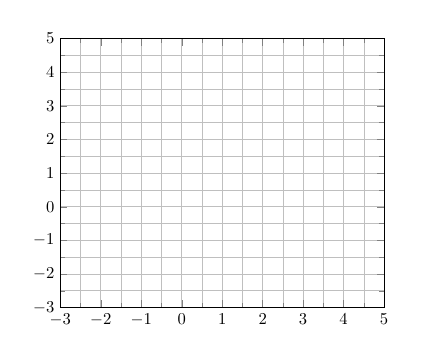
\begin{tikzpicture}[scale=0.6]
\begin{axis}[grid=both, ymin=-3,ymax=5,xmax=5,xmin=-3,xtick={-4,-3,...,5},ytick={-3,-2,...,5},minor tick num=1,
]             
  \end{axis}
\end{tikzpicture}
\end{center}
\end{minipage}
\end{minipage}

\begin{solution}

\begin{minipage}{\textwidth}
\begin{minipage}{0.6\textwidth}
\begin{enumerate}[label={(\arabic*)},afterlabel=\quad]
\item
 The line of symmetry is $x=\h$. The $x$-intercepts are $(\rtwo, 0)$ and $(\rone,0)$. The $y$-intercept is $(0, \c)$. The vertex is $(\h, -\k)$.
\item The graph of $f$ is shown in the right.
\end{enumerate}
\end{minipage}
\begin{minipage}{0.4\textwidth}
\begin{center}
\begin{tikzpicture}[scale=0.6]
\begin{axis}[grid=both, ymin=-3,ymax=5,xmax=5,xmin=-3,xtick={-4,-3,...,5},ytick={-3,-2,...,5},minor tick num=1]     
 \addplot[thick, samples=100]   {(x-\h)^2-\k};         
  \end{axis}
\end{tikzpicture}
\end{center}
\end{minipage}
\end{minipage}
\end{solution}

